% Select legacy T1 fonts before IEEEtran initializes its Times font metrics.
% This also avoids TU/ptm substitutions in Unicode engines such as Tectonic.
\renewcommand{\rmdefault}{ptm}
\RequirePackage[T1]{fontenc}
\documentclass[conference]{IEEEtran}
\usepackage[utf8]{inputenc}
\usepackage{graphicx}
\usepackage{float}
\usepackage{booktabs}
\usepackage{array}
\usepackage{ragged2e}
\usepackage{url}
\usepackage{xurl}
\usepackage{microtype}
\usepackage{multirow}
\usepackage{tabularx}
\usepackage{placeins}
\usepackage{amssymb}
\newcolumntype{P}[1]{>{\RaggedRight\arraybackslash}p{#1}}
\newcolumntype{Y}{>{\RaggedRight\arraybackslash}X}
\usepackage{amsmath}
\usepackage{siunitx}
\usepackage{flushend}
\usepackage{dblfloatfix}
\usepackage{cite}
\usepackage{enumitem}
\setlist{nosep,leftmargin=*}
\renewcommand{\figurename}{Gambar}
\renewcommand{\tablename}{Tabel}
\graphicspath{{assets/}}

% Revisi penulisan: data, scaler, assignment, dan model Stage 3 tidak diubah.
% Keputusan penulis yang belum disahkan dicatat pada AUDIT_PERUBAHAN.md.

\begin{document}

\title{Klasterisasi Kondisi Operasi Turbin Angin Kelmarsh Menggunakan K-Means++ pada Representasi Temporal SCADA Multivariat}

\author{%
\begin{tabular}{ccc}
\begin{tabular}{c}
\sublargesize Alfon Darren Witanto\\
\itshape\normalsize dept. Ilmu Komputer\\
\itshape\normalsize Universitas Padjadjaran\\
\normalfont\normalsize Sumedang, Indonesia\\
\normalfont\normalsize alfon24001@mail.unpad.ac.id
\end{tabular}
&
\begin{tabular}{c}
\sublargesize Dean Frederic Wijaya\\
\itshape\normalsize dept. Ilmu Komputer\\
\itshape\normalsize Universitas Padjadjaran\\
\normalfont\normalsize Sumedang, Indonesia\\
\normalfont\normalsize dean24001@mail.unpad.ac.id
\end{tabular}
&
\begin{tabular}{c}
\sublargesize Hansel Stevan Boike\\
\itshape\normalsize dept. Ilmu Komputer\\
\itshape\normalsize Universitas Padjadjaran\\
\normalfont\normalsize Sumedang, Indonesia\\
\normalfont\normalsize hansel24001@mail.unpad.ac.id
\end{tabular}
\\[1.5em]
\multicolumn{3}{c}{%
\begin{tabular}{cc}
\begin{tabular}{c}
\sublargesize Syamil Azzimul Bashry\\
\itshape\normalsize dept. Ilmu Komputer\\
\itshape\normalsize Universitas Padjadjaran\\
\normalfont\normalsize Sumedang, Indonesia\\
\normalfont\normalsize syamil24004@mail.unpad.ac.id
\end{tabular}
&
\begin{tabular}{c}
\sublargesize Valensius Alven\\
\itshape\normalsize dept. Ilmu Komputer\\
\itshape\normalsize Universitas Padjadjaran\\
\normalfont\normalsize Sumedang, Indonesia\\
\normalfont\normalsize valensius24001@mail.unpad.ac.id
\end{tabular}
\end{tabular}}
\end{tabular}}

\maketitle
\raggedbottom

\begin{abstract}
Penelitian ini mengklasterkan kondisi operasi tanpa label pada SCADA enam turbin Kelmarsh 2022. Dari 315.360 slot 10 menit, 314.018 observasi tersedia. Preprocessing berbasis benchmark mempertahankan ekstrem berflag, mengisi 19 sel ambien, dan menghasilkan 52.241 window satu jam dengan 60 fitur statistik dari 11 variabel fisik; standardisasi ditetapkan pada Januari--Juni dan Juli--Desember dipakai untuk seleksi, bukan pengujian independen. K-Means++, Fuzzy C-Means, HDBSCAN, dan Ward diuji pada $k=2$--10. K-Means++ $k=2$ memperoleh Silhouette 0,32954, Davies--Bouldin 1,85605, dan Calinski--Harabasz 4071,28; FCM degeneratif dan HDBSCAN memberi inti padat dengan cakupan parsial. Refit deskriptif menghasilkan dua kelompok (10.405 dan 41.836 window) yang dibedakan oleh daya, putaran, dan pitch, bukan label fault. Kontrol terkendali menunjukkan pilihan skala paling menentukan struktur, sedangkan representasi temporal menstabilkan label.
\end{abstract}
\begin{IEEEkeywords}
SCADA, Kelmarsh, preprocessing, K-Means++, klasterisasi temporal.
\end{IEEEkeywords}

\section{Pendahuluan}
SCADA (Supervisory Control and Data Acquisition) turbin merekam besaran mekanik, listrik, termal, dan lingkungan dengan satuan serta dinamika berbeda. Dataset Kelmarsh menyediakan deret multivariat 10 menit tanpa label kondisi operasi \cite{kelmarsh2025}. Klasterisasi berbasis jarak menghadapi ketimpangan skala, redundansi, celah, arah sirkular, dan ekstrem yang belum tentu merupakan kesalahan. Memetakan kelompok yang dapat ditelusuri secara fisik membutuhkan audit preprocessing sekaligus pemeriksaan struktur kelompok, bukan hanya skor internal.

Studi temporal memakai window, kompresi, atau struktur korelasi \cite{martipuig2024,bonifati2022,bette2023}; perbandingan sensor gedung \cite{ngophan2025} serta studi forecasting angin \cite{cai2025} memberi primitif berbeda. Penelitian ini bertujuan menetapkan input temporal yang konsisten, membandingkan keluarga klasterisasi pada input yang tetap, dan mendeskripsikan kelompok beserta batas interpretasinya. Perbandingan kausal antarstrategi preprocessing dan representasi temporal versus per-observasi dilaporkan sebagai kontrol tambahan.

Kontribusi kelompok mencakup tiga hal: (i) integrasi benchmark preprocessing Kelmarsh yang dapat ditelusuri, (ii) perbandingan HDBSCAN pada populasi evaluasi yang disamakan, serta (iii) profil fisik dan kontinuitas temporal dari model deskriptif tanpa label.

\subsection{Seleksi literatur, diagram PRISMA-ScR, dan gap}
Seleksi literatur mengikuti alur Preferred Reporting Items for Systematic Reviews and Meta-Analyses for Scoping Reviews (PRISMA-ScR). Penelusuran Scopus pada 1 Oktober 2026 menghasilkan 766 dokumen; filter tahun 2021--2026 menyisakan 474, lalu 202 akses terbuka, 201 berbahasa Inggris, 164 artikel, dan 103 setelah filter domain. Sebelas studi diambil sebagai set sintesis kerja. Gambar~\ref{fig:prisma} menyajikan alur seleksi ini; statusnya merupakan audit kerja, bukan klaim inklusi PRISMA final.

\begin{figure}[H]
\centering
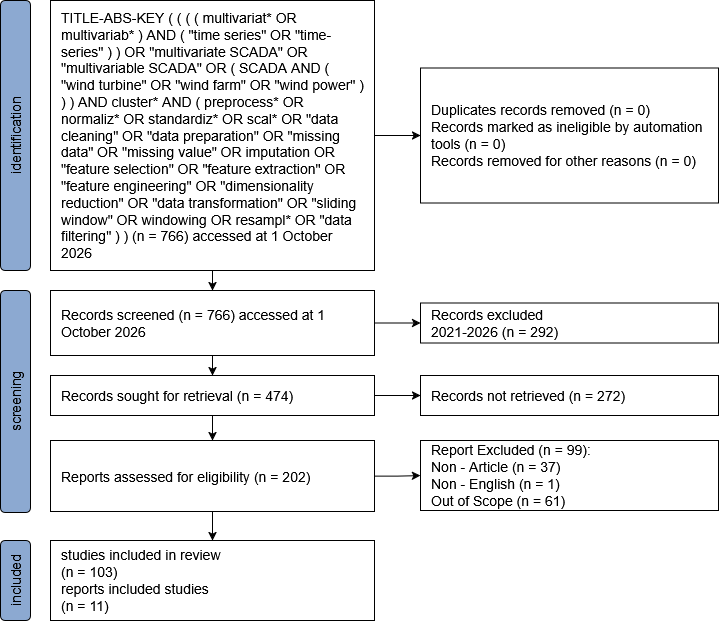
\includegraphics[width=0.66\columnwidth]{prisma_scr.png}
\caption{Diagram alir seleksi studi berdasarkan PRISMA-ScR.}
\label{fig:prisma}
\end{figure}

% Gap Analysis table: No | Paper | Domain | Clustering | Preprocessing | Limitasi/Kesenjangan.
\begin{table*}[!t]
\centering
\caption{Gap Analysis sebelas paper sintesis kerja.}
\label{tab:gap}
\scriptsize
\setlength{\tabcolsep}{2.5pt}
\renewcommand{\arraystretch}{0.98}
\begin{tabularx}{\textwidth}{@{}P{.02\textwidth}P{.11\textwidth}P{.135\textwidth}P{.125\textwidth}P{.145\textwidth}Y@{}}
\toprule
\textbf{No} & \textbf{Paper} & \textbf{Domain} & \textbf{Clustering} & \textbf{Preprocessing} & \textbf{Limitasi dan/atau Kesenjangan yang Diselesaikan Paper} \\
\midrule
1 & Marti-Puig dan N\'{u}\~{n}ez-Vilaplana \cite{martipuig2024} & SCADA turbin angin (5 turbin, 5 menit) & Hierarkis aglomeratif pada window & Window bergeser; transformasi kosinus diskret (DCT) & Mengelompokkan turbin per window temporal; sinyal tunggal dan DCT membatasi transfer ke statistik multivariat, dan jumlah klaster berubah tiap frame. \\
2 & Bonifati dkk. \cite{bonifati2022} & MTS umum (18 dataset UEA) & K-Means berbasis fitur & Fitur intra/inter-sinyal; cleaning; normalisasi; seleksi PFA & Representasi fitur bernama mendukung interpretasi; ribuan fitur dan Principal Feature Analysis (PFA) berbeda dari 60 statistik dan mengaburkan keterlacakan ke sensor. \\
3 & Ngo dan Phan \cite{ngophan2025} & Sensor gedung dalam ruangan & K-Means/DTW, HDBSCAN, K-Shape, SOM & Normalisasi Min--Max; turunan pertama & Membandingkan banyak algoritma dan validitas internal; hasil khusus domain gedung sehingga tak menjamin rezim turbin dan tak menyediakan label operasi. \\
4 & Mazgu\l{}a dkk. \cite{mazgula2024} & KPI 5G + akselerometer & Spectral dengan DTW terbatas & Standardisasi; moving average & Menyetarakan skala berbeda via standardisasi; jarak DTW berbeda dari Euclidean pada statistik window dan smoothing meredam transisi operasi. \\
5 & Cai dkk. \cite{cai2025} & SCADA angin lepas pantai + NWP & Optimized FCM; pengelompokan tren & Penanganan missing/outlier; seleksi fitur; scaling & Menangani missing/outlier untuk forecasting; sasaran prediksi dan FCM teroptimasi tidak sama dengan pengelompokan deskriptif tanpa label. \\
6 & Ghaderi dkk. \cite{ghaderi2023} & Deret waktu klinis (TBI) & SLAC-Time berbasis pembelajaran mandiri & Observation triplets; window; tanpa imputasi konvensional & Menghindari imputasi konvensional lewat observation triplet; arsitektur dan interval tidak teratur tidak diterapkan pada SCADA 10 menit yang teratur. \\
7 & Draayer dkk. \cite{draayer2026} & Sinyal sensor umum (EEG, gerak) & Deep clustering untuk segmentasi & Subsequence; autoencoder; augmentasi & Menemukan segmen homogen lewat representasi neural; pelatihan embedding mengubah ruang fitur dan menambah biaya komputasi. \\
8 & Bel-Hadj dkk. \cite{belhadj2026} & Vibrasi nacelle turbin angin lepas pantai & Deep Embedded Clustering; K-Means inisialisasi & Spektrum akselerasi; percentile scaling; denoising & Menafsirkan kondisi operasi turbin; modalitas akselerasi frekuensi tinggi berbeda resolusi dari SCADA 10 menit. \\
9 & Lang dkk. \cite{lang2026} & Monitoring operasi kapal (tanker, 1 Hz) & Toeplitz Inverse Covariance-based Clustering (TICC) & Averaging 15 menit; window; change-point & Menyegmentasi stream multivariat dengan konsistensi waktu; agregasi dapat melebur kejadian pendek dan domain kapal berbeda dari turbin. \\
10 & Bette dkk. \cite{bette2023} & SCADA turbin angin lepas pantai frekuensi tinggi & Klasterisasi matriks korelasi & Averaging; epoch 30 menit; Z-score; Pearson & Menunjukkan struktur korelasi berubah menurut angin dan kontrol; matriks korelasi epoch bukan 60 statistik window, sehingga representasi tidak langsung dipindahkan. \\
11 & Li dan Li \cite{li2026} & SCADA turbin angin onshore (anomali) & VGO-K-Means; pembanding K-Means/DBSCAN & Statistik $3\sigma$; Z-score; variable grid & Menapis anomali lewat grid variabel dan Z-score; tujuan penapisan berbeda dari pemetaan seluruh window dan bukan replikasi K-Means++. \\
\bottomrule
\end{tabularx}
\par\vspace{2pt}
{\footnotesize\textit{Catatan:} DTW menyelaraskan dua deret; K-Shape memakai kemiripan bentuk; SOM memetakan objek ke kisi prototipe; spectral clustering memakai eigenvektor graf; autoencoder dan DEC adalah representasi neural; pembelajaran mandiri memperoleh sinyal latihan dari data sendiri; TICC memakai kovariansi Toeplitz antarwaktu; change-point menandai perubahan distribusi. Istilah ini pembanding di luar cakupan, bukan eksperimen Kelmarsh.\par}
\end{table*}

Kesenjangan yang disasar adalah belum tersedianya representasi multivariat-temporal dan protokol evaluasi yang konsisten untuk SCADA Kelmarsh, sehingga perbandingan keluarga klasterisasi kerap bercampur dengan perubahan preprocessing. Tabel~\ref{tab:gap} merangkum sebelas paper sintesis kerja beserta domain data, metode klasterisasi, preprocessing, dan kesenjangan yang diselesaikannya.

Tabel~\ref{tab:gap} menunjukkan primitif yang dapat dipindahkan, tetapi metode domain lain tidak menjamin hasil yang sama. Baris 7--11 memperlihatkan batas modalitas dan representasi: spektrum akselerasi \cite{belhadj2026}, embedding neural \cite{draayer2026}, TICC \cite{lang2026}, dan matriks korelasi \cite{bette2023} berbeda dari 60 statistik Kelmarsh. Karena itu transfer dilakukan melalui benchmark lokal; optimizer dan model yang tidak dijalankan tetap dibedakan dari metode aktual.

\section{Metodologi preprocessing dan pemodelan}
\subsection{Alur perancangan}
Gambar~\ref{fig:workflow} merangkum alur kerja dari data mentah hingga profil deskriptif. Preprocessing dibekukan sebelum klasterisasi sehingga seluruh kandidat menerima input identik; cabang kontrol memisahkan pengaruh pilihan preprocessing dari pengaruh algoritma.

\begin{figure}[!t]
\centering
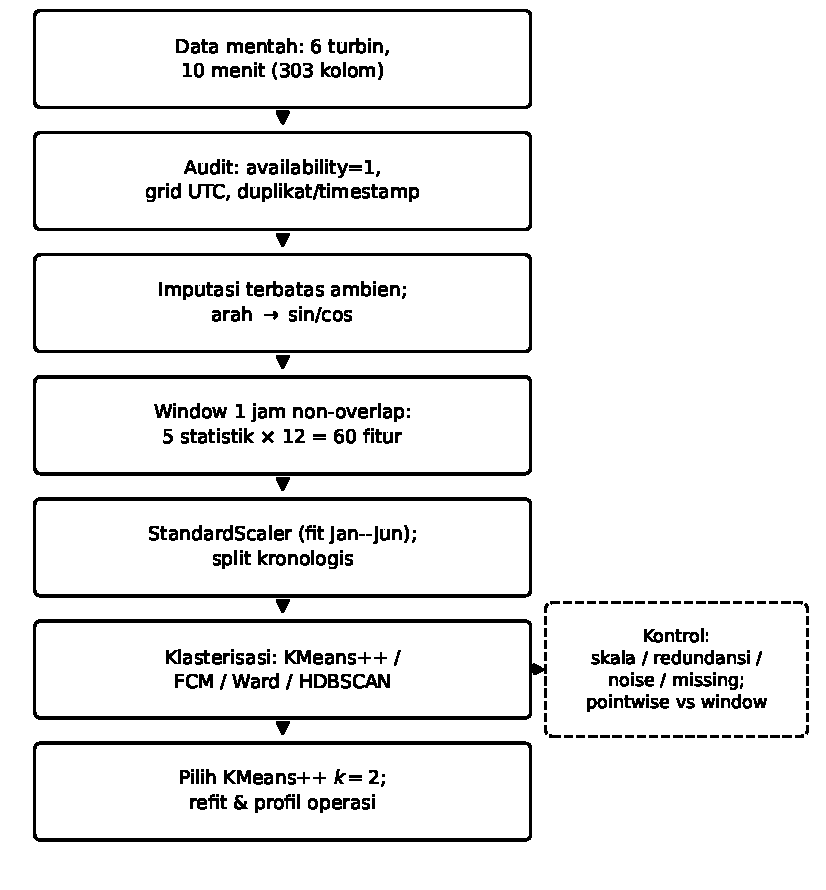
\includegraphics[width=0.64\columnwidth]{workflow.pdf}
\caption{Alur kerja preprocessing, klasterisasi, dan kontrol.}
\label{fig:workflow}
\end{figure}

\subsection{Data, audit, dan imputasi terbatas}
Enam turbin Senvion MM92 berdaya 2.050 kW/unit pada Kelmarsh versi 4 \cite{kelmarsh2025} dipetakan ke grid UTC tahun 2022. Availability=1 menyatakan observasi tersedia. Dari 302 kolom numerik dipilih 11 sinyal fisik yang dapat ditelusuri \cite{bonifati2022,bette2023,li2026}: angin/arah, daya aktif/reaktif, ambien, bearing generator depan, oli gearbox, rotor/generator, pitch blade A, dan frekuensi. Setpoint, waktu, identitas, flag, dan event hanya konteks. Fit menggunakan Januari--Juni; Juli--Desember untuk seleksi. Split kronologis adalah keputusan Kelmarsh, dengan pertimbangan missing-data dari \cite{ghaderi2023}, bukan final test independen.

\begin{table}[!t]
\centering
\caption{Rincian kumpulan data Kelmarsh 2022.}
\label{tab:dataset}
\footnotesize
\setlength{\tabcolsep}{4pt}
\begin{tabular}{lr}
\toprule
Aspek & Nilai \\
\midrule
Turbin (Senvion MM92) & 6 \\
Daya terpasang per turbin & 2.050 kW \\
Periode (UTC) & 2022, interval 10 menit \\
Slot terjadwal & 315.360 \\
Observasi tersedia & 314.018 \\
Kolom mentah (numerik) & 303 (302) \\
Sinyal fisik dipakai & 11 \\
Koordinat model & 12 \\
Fitur per window & 60 \\
Window final & 52.241 \\
\quad training (Jan--Jun) & 25.881 \\
\quad seleksi (Jul--Des) & 26.360 \\
Sel missing terisi & 19 (ambien) \\
\bottomrule
\end{tabular}
\end{table}

\textit{Pearson correlation} menilai hubungan linear untuk pasangan valid $\mathcal I$ \cite{bette2023,bonifati2022}:
\begin{equation}
r_{xy}=\frac{\sum_{i\in\mathcal I}(x_i-\bar x)(y_i-\bar y)}{\sqrt{\sum_{i\in\mathcal I}(x_i-\bar x)^2\sum_{i\in\mathcal I}(y_i-\bar y)^2}}.
\label{eq:pearson}
\end{equation}
$x_i,y_i$ ialah nilai dua sensor; $\bar x,\bar y$ mean pasangan valid. Spearman adalah korelasi peringkat; autokorelasi memasangkan sinyal dengan dirinya pada lag waktu nyata, tanpa menyambung gap.

\textit{Imputasi}, pengisian nilai hilang, mengadaptasi primitif \cite{bonifati2022,cai2025,ghaderi2023}. Benchmark tersimpan membandingkan penghapusan, median training, forward fill, linear, spline, KNN, dan mean turbin pada gap buatan 1/2/6/18 slot. Gate Kelmarsh menerima nRMSE $\leq0,10$ pada 1--2 slot, pengisian $\geq99\%$, dan tidak lebih buruk daripada median/forward fill. nRMSE adalah akar mean galat kuadrat ternormalisasi IQR training (simpangan baku bila IQR tidak positif; lalu 1 bila tidak valid). Median ialah nilai tengah; IQR ialah selisih kuartil ketiga dan pertama. Forward fill memakai nilai teramati terakhir; KNN (k-nearest neighbors) mengisi dari tetangga terdekat; spline memakai kurva polinomial tersambung. Hanya ambien lolos. Interpolasi linear menghubungkan dua batas dengan garis lurus:
\begin{equation}
\hat x(t)=x(t_L)+\frac{t-t_L}{t_R-t_L}[x(t_R)-x(t_L)],
\label{eq:linear}
\end{equation}
dengan $t_L,t_R$ batas teramati, $t_L<t<t_R$, $x$ ambien, dan $\hat x$ pengisian. Seluruh run hilang harus 1--2 slot (20 menit nilai hilang); run lebih panjang tidak diisi sebagian. Turbin/split tidak dilintasi. Dua slot hilang mempunyai batas teramati berselisih 30 menit; hanya 19 sel aktual diisi.

Penanganan ekstrem mengadaptasi \cite{ngophan2025,cai2025,li2026,belhadj2026}. IQR trimming (penghapusan di luar pagar kuartil), z-score trimming (penghapusan menurut jarak dari mean dalam unit std), winsorization (pembatasan ekstrem), DBSCAN (Density-Based Spatial Clustering of Applications with Noise, penapisan kepadatan), dan replacement regresi mempunyai benchmark tersimpan. Kebijakan akhir \textit{flag-only}: nilai tetap, tanpa trimming/replacement. Rentang fisik adalah heuristik audit, bukan batas pabrikan; arah di luar rentang tidak dikodekan. Flag bukan fitur atau label fault.

\subsection{Standardisasi, arah sirkular, dan window}
\textit{StandardScaler} mengadaptasi penyetaraan antar-satuan \cite{mazgula2024,bette2023,li2026}:
\begin{equation}
z_{ij}=\frac{x_{ij}-\mu_j}{\sigma_j},\qquad
\sigma_j^2=\frac{1}{N_T}\sum_{i\in\mathcal T}(x_{ij}-\mu_j)^2.
\label{eq:zscore}
\end{equation}
$j$ indeks fitur; $\mathcal T$ training, $N_T=|\mathcal T|$, dan $\mu_j$ mean training. Pembagi adalah $N_T$ (ddof=0); skala nol diganti 1. Median training mengisi nilai kosong untuk fit scaler benchmark titik, tanpa menjadikannya pengukuran final. Global Standard dipilih terhadap Min--Max (minimum/rentang) dan Robust (median/IQR); parameter dibekukan untuk seleksi.

\textit{Circular encoding} mengadaptasi representasi arah \cite{cai2025,lang2026}, dengan sudut $\theta(t)$ dalam derajat:
\begin{equation}
d_{\sin}(t)=\sin\frac{\pi\theta(t)}{180},\quad d_{\cos}(t)=\cos\frac{\pi\theta(t)}{180}.
\label{eq:circular}
\end{equation}
$d_{\sin},d_{\cos}$ ialah koordinat arah tanpa satuan; sudut melingkar menyamakan $0^\circ$ dan $360^\circ$. Sepuluh skalar dan pasangan arah menghasilkan 12 koordinat. Sin/cos titik memakai skala unit sama; untuk setiap statistik window, skala pasangan diganti akar rata-rata kuadrat kedua skala training, dengan mean tetap per koordinat.

\textit{Window non-overlap} adalah interval tanpa tumpang tindih \cite{martipuig2024,bonifati2022,lang2026,bette2023}. Aturan benchmark memilih durasi terpendek dengan retensi seleksi $\geq80\%$, lalu kelengkapan paling ketat; terpilih satu jam, $L=6$ slot lengkap. Untuk nilai berurutan $v_{w\ell j}$ dalam window $w$, lima statistik mengikuti representasi bernama \cite{bonifati2022}:
\begin{align}
\bar v_{wj}&=\frac{1}{L}\sum_{\ell=1}^{L}v_{w\ell j},\quad
s_{wj}=\sqrt{\frac{\sum_{\ell=1}^{L}(v_{w\ell j}-\bar v_{wj})^2}{L-1}},\label{eq:windowstats}\\
v^{\min}_{wj}&=\min_\ell v_{w\ell j},\quad v^{\max}_{wj}=\max_\ell v_{w\ell j},\nonumber\\
\Delta v_{wj}&=v_{wLj}-v_{w1j}.\label{eq:endpoint}
\end{align}
$\ell=1,\ldots,L$ adalah urutan slot; $\bar v,s,v^{\min},v^{\max},\Delta v$ ialah mean, std sampel (ddof=1), minimum, maksimum, dan perubahan endpoint (selisih, bukan slope/jam). Statistik dibentuk dari nilai fisik setelah interpolasi diterima dan pasangan arah, bukan kolom scalar-scaled titik. Enam puluh statistik distandardisasi tersendiri pada window training, dengan shared scale sin/cos per statistik. Median/flag imputasi koordinat disimpan sebagai pengaman. Urutan fitur, scaler, dan SHA-256 input tetap untuk semua kandidat. PCA (proyeksi), DCT (kompresi frekuensi), tsfresh (ekstraksi otomatis), PFA (seleksi fitur asli), serta smoothing/derivative hanya diagnostik alternatif, tidak pada input utama \cite{bonifati2022,martipuig2024}.

\subsection{Kandidat klasterisasi yang telah dijalankan}
Dalam pemodelan, $\mathcal T$ dan $N_T$ merujuk window training. Tuliskan $\mathbf x_i\in\mathbb R^{60}$ sebagai vektor window terstandar; $C_j$ klaster, $k$ jumlah diminta, dan $\mathbf c_j$ centroid.
\textit{K-Means} meminimalkan kuadrat jarak Euclidean:
\begin{equation}
J_{\mathrm{KM}}=\sum_{j=1}^{k}\sum_{i\in C_j}\|\mathbf x_i-\mathbf c_j\|_2^2.
\label{eq:kmeans}
\end{equation}
$\mathbf c_j$ mean anggota $C_j$ dan $\|\cdot\|_2$ norma Euclidean. Baseline berbasis fitur mengikuti \cite{bonifati2022,ngophan2025}; seeding K-Means++ berbobot jarak kuadrat memakai varian greedy scikit-learn. Konfigurasi aktual $k=2$--10, Lloyd, 20 inisialisasi, 500 iterasi maksimum, toleransi relatif perpindahan pusat $10^{-4}$, seed 2022; lima seed 2022--2026 mengaudit stabilitas tiap $k$.

\textit{Fuzzy C-Means} (FCM) memberi keanggotaan beberapa pusat:
\begin{equation}
J_m=\sum_{i=1}^{N_T}\sum_{j=1}^{k}u_{ij}^{m}\|\mathbf x_i-\mathbf c_j\|_2^2.
\label{eq:fcm}
\end{equation}
$u_{ij}\in[0,1]$, $\sum_j u_{ij}=1$, dan fuzzifier $m>1$ mengatur kekaburan. FCM standar menguji soft assignment \cite{cai2025}, tanpa optimizer/forecasting mereka. Scikit-fuzzy memakai $m=2$, $k=2$--10, lima seed, 500 iterasi maksimum, serta penghentian $\|U^{(r+1)}-U^{(r)}\|_F<10^{-5}$ ($U$ matriks keanggotaan, $r$ iterasi, norma Frobenius). Inisialisasi konvergen dipilih berdasarkan objektif training; pusat tetap memberi keanggotaan seleksi dan hard label $\arg\max_j u_{ij}$. FPC, jumlah kuadrat keanggotaan dibagi banyak objek, mendekati $1/k$ bila seragam; entropi ternormalisasi mendekati 1. Ambiguitas memakai $\max_j u_{ij}<0,60$.

\textit{HDBSCAN}, hierarki kepadatan dengan label noise \cite{ngophan2025}, menguji enam kombinasi minimum klaster $100/300/800$ dan minimum sampel $10/30$ pada semua training. Pustaka hdbscan 0.8.44 memakai Euclidean, \texttt{prims\_kdtree}, excess-of-mass, dan prediction data. Jumlah kelompok tidak dikendalikan $k$. Approximate prediction seleksi memakai struktur training tetap, tanpa kelompok baru; noise $-1$ disimpan.

\textit{Agglomerative Ward} menggabungkan $A,B$ dengan kenaikan kuadrat intraklaster terkecil:
\begin{equation}
\Delta J(A,B)=\frac{|A||B|}{|A|+|B|}\|\mathbf c_A-\mathbf c_B\|_2^2.
\label{eq:ward}
\end{equation}
$|A|,|B|$ jumlah anggota, $\mathbf c_A,\mathbf c_B$ centroid. Keluarga hierarkis dimotivasi \cite{martipuig2024}, tetapi linkage adalah keputusan Kelmarsh. $k=2$--10 memakai 4.000 training deterministik karena memori; K-Means pembanding di-fit pada sampel sama. Tidak ada prediksi seleksi Ward. GMM tidak dijalankan karena justifikasi empiris tambahan belum ditetapkan.

\subsection{Rancangan kontrol dan representasi}
Untuk memisahkan pengaruh pilihan preprocessing dari algoritma, dilakukan kontrol satu faktor: satu keputusan diubah sementara sisanya tetap pada konfigurasi referensi (StandardScaler, 60 statistik, tanpa pembatasan ekstrem, missing ambien-terbatas) dengan K-Means++ $k=2$, seed, dan fitur yang sama. Setiap varian dinilai dengan Silhouette, DBI, dan CHI, ditambah \textit{Adjusted Rand Index} (ARI), yaitu kesesuaian partisi terkoreksi peluang; ARI mendekati 1 berarti struktur hampir tidak berubah dan mendekati 0 berarti partisi berbeda. Ukuran klaster terkecil, stabilitas seed, dan persistence juga dicatat agar skor tinggi akibat kelompok mungil dapat dikenali.

Faktor skala membandingkan tanpa scaling, StandardScaler (referensi), \textit{RobustScaler} (median dan IQR, lebih tahan pencilan), \textit{Min--Max} (pemetaan linear ke $[0,1]$), dan standardisasi per-turbin; primitif penyetaraan skala mengikuti \cite{mazgula2024,li2026,bette2023}, sedangkan pemilihan dan penolakan varian merupakan keputusan benchmark Kelmarsh. Faktor redundansi membandingkan 60 statistik (referensi) dengan hanya 12 mean koordinat, pembuangan keluarga generator, representasi level-tambah-dinamika, dan pembuangan keluarga frekuensi; motivasi menghapus fitur derived dan redundan mengikuti \cite{bonifati2022,li2026,bette2023}. Faktor ekstrem membandingkan tanpa pembatasan dengan \textit{winsorization}, yaitu pembatasan nilai ke persentil, pada $1$--$99$ dan $5$--$95$ \cite{cai2025,belhadj2026}. Faktor missing membandingkan kebijakan ambien-terbatas (referensi), pembuangan baris (\textit{listwise}), median training, dan forward fill \cite{bonifati2022,cai2025,ghaderi2023}.

Kontrol representasi temporal membandingkan klasterisasi observasi 10 menit individual (pointwise) dengan window satu jam pada 12 sinyal, scaler, split, dan algoritma yang sama, sehingga perbedaan bersumber dari agregasi temporal; gagasan window versus observasi tunggal dimotivasi \cite{martipuig2024,draayer2026,lang2026}. Selain indeks internal, diukur koherensi temporal berupa panjang run (rata-rata dan median durasi label bertahan, dalam jam), laju pergantian label per jam, dan ARI antara label window dan label pointwise setelah label window dipetakan ke enam observasi anggotanya.

\subsection{Validitas, kontinuitas, dan pemilihan}
Pada populasi evaluasi $E$, \textit{Silhouette} adalah mean
\begin{equation}
s_i=\frac{b_i-a_i}{\max(a_i,b_i)},
\label{eq:silhouette}
\end{equation}
$a_i$ mean jarak ke anggota klaster sendiri di $E$ dan $b_i$ mean jarak minimum ke klaster lain; singleton diberi nol. Untuk K-Means/FCM, $E$ adalah 3.000 seleksi deterministik; jarak dihitung di dalam sampel, bukan semua 26.360. HDBSCAN dan K-Means matched memakai irisan sampel dengan non-noise yang sama; Ward memakai 3.000 dari sampel training bersama.

\textit{Davies--Bouldin Index} mengukur rasio sebaran/pemisahan:
\begin{equation}
\mathrm{DBI}=\frac{1}{K}\sum_{j=1}^{K}\max_{h\ne j}\frac{S_j+S_h}{\|\mathbf c_j-\mathbf c_h\|_2}.
\label{eq:dbi}
\end{equation}
$K$ jumlah label terisi; $S_j$ mean jarak objek ke centroid klaster $j$. \textit{Calinski--Harabasz Index} membandingkan dispersi:
\begin{equation}
\mathrm{CHI}=\frac{\sum_j n_j\|\mathbf c_j-\bar{\mathbf x}\|_2^2/(K-1)}{\sum_j\sum_{i\in C_j}\|\mathbf x_i-\mathbf c_j\|_2^2/(N-K)}.
\label{eq:chi}
\end{equation}
$n_j=|C_j|$, $N$ ukuran populasi, dan $\bar{\mathbf x}$ mean seluruh populasi. DBI/CHI memakai seleksi penuh, non-noise matched, atau 4.000 training sesuai eksperimen. Silhouette/CHI lebih tinggi dan DBI lebih rendah dibaca pada populasi sebanding; indeks tidak dipakai bila label terisi tidak cukup.

\textit{Adjusted Rand Index} (ARI) menilai kesesuaian partisi terkoreksi peluang; Normalized Mutual Information (NMI) menilai asosiasi label dengan identitas/flag, bukan akurasi operasi. Temporal persistence, diagnostik kontinuitas yang dimotivasi \cite{lang2026}, adalah
\begin{equation}
P=\frac{1}{|\mathcal A|}\sum_{(i,h)\in\mathcal A}\mathbf1[g(i)=g(h)].
\label{eq:persistence}
\end{equation}
$g(i)$ label; $\mathbf1$ indikator; $\mathcal A$ pasangan pada turbin dan split sama, tepat satu jam, tanpa melintasi gap. HDBSCAN all-label dan assigned-only mempunyai penyebut berbeda. Pemilihan mempertimbangkan indeks \cite{ngophan2025,li2026}, kelompok kecil (peringatan $<1\%$), seed, kontinuitas, profil, dan cakupan. Refit seluruh tahun yang sudah tersedia dilakukan setelah pemeriksaan kandidat, dengan scaler training tetap; profil refit dipisahkan dari skor seleksi.



\section{Hasil dan pembahasan}
\subsection{Statistik deskriptif dan ketergantungan temporal}
Tabel~\ref{tab:desc} merangkum statistik deskriptif sinyal terpilih pada baris tersedia. Skewness, yaitu kemiringan distribusi (0 simetris, $>0$ ekor kanan, $<0$ ekor kiri), menandai beberapa sinyal tidak simetris: frekuensi $-118,80$, oli $-2,63$, dan pitch $+2,62$. Nilai ini menandakan beberapa kondisi operasi (diam, normal, rated), sehingga mean dan std dibaca hati-hati dan median/IQR menjadi pertimbangan. Gambar~\ref{fig:quantiles} menampilkan sebaran kuantil tiap sinyal; ekor panjang pada daya dan pitch sejalan dengan kebijakan mempertahankan ekstrem berflag \cite{ngophan2025,cai2025,li2026,belhadj2026} alih-alih trimming.

\begin{table}[!t]
\centering
\caption{Statistik deskriptif sinyal terpilih pada baris tersedia ($n=314.018$).}
\label{tab:desc}
\footnotesize
\setlength{\tabcolsep}{3pt}
\begin{tabular}{lrrrr}
\toprule
Sinyal & Mean & Std & Skew & Missing \% \\
\midrule
Angin (m/s) & 5,95 & 2,69 & 0,65 & 0,000 \\
Daya (kW) & 559,55 & 593,34 & 1,10 & 0,000 \\
Reaktif (kvar) & $-190,52$ & 171,53 & $-0,87$ & 0,000 \\
Ambien ($^\circ$C) & 12,19 & 6,17 & 0,40 & 0,082 \\
Bearing ($^\circ$C) & 37,83 & 7,47 & $-1,83$ & 0,000 \\
Oli ($^\circ$C) & 51,25 & 9,68 & $-2,63$ & 0,000 \\
Rotor (RPM) & 9,88 & 4,55 & $-0,95$ & 0,000 \\
Generator (RPM) & 1172,18 & 538,15 & $-0,95$ & 0,000 \\
Pitch (derajat) & 9,56 & 22,51 & 2,62 & 0,082 \\
Frekuensi (Hz) & 49,99 & 0,36 & $-118,80$ & 0,000 \\
\bottomrule
\end{tabular}
\end{table}

\begin{figure}[H]
\centering
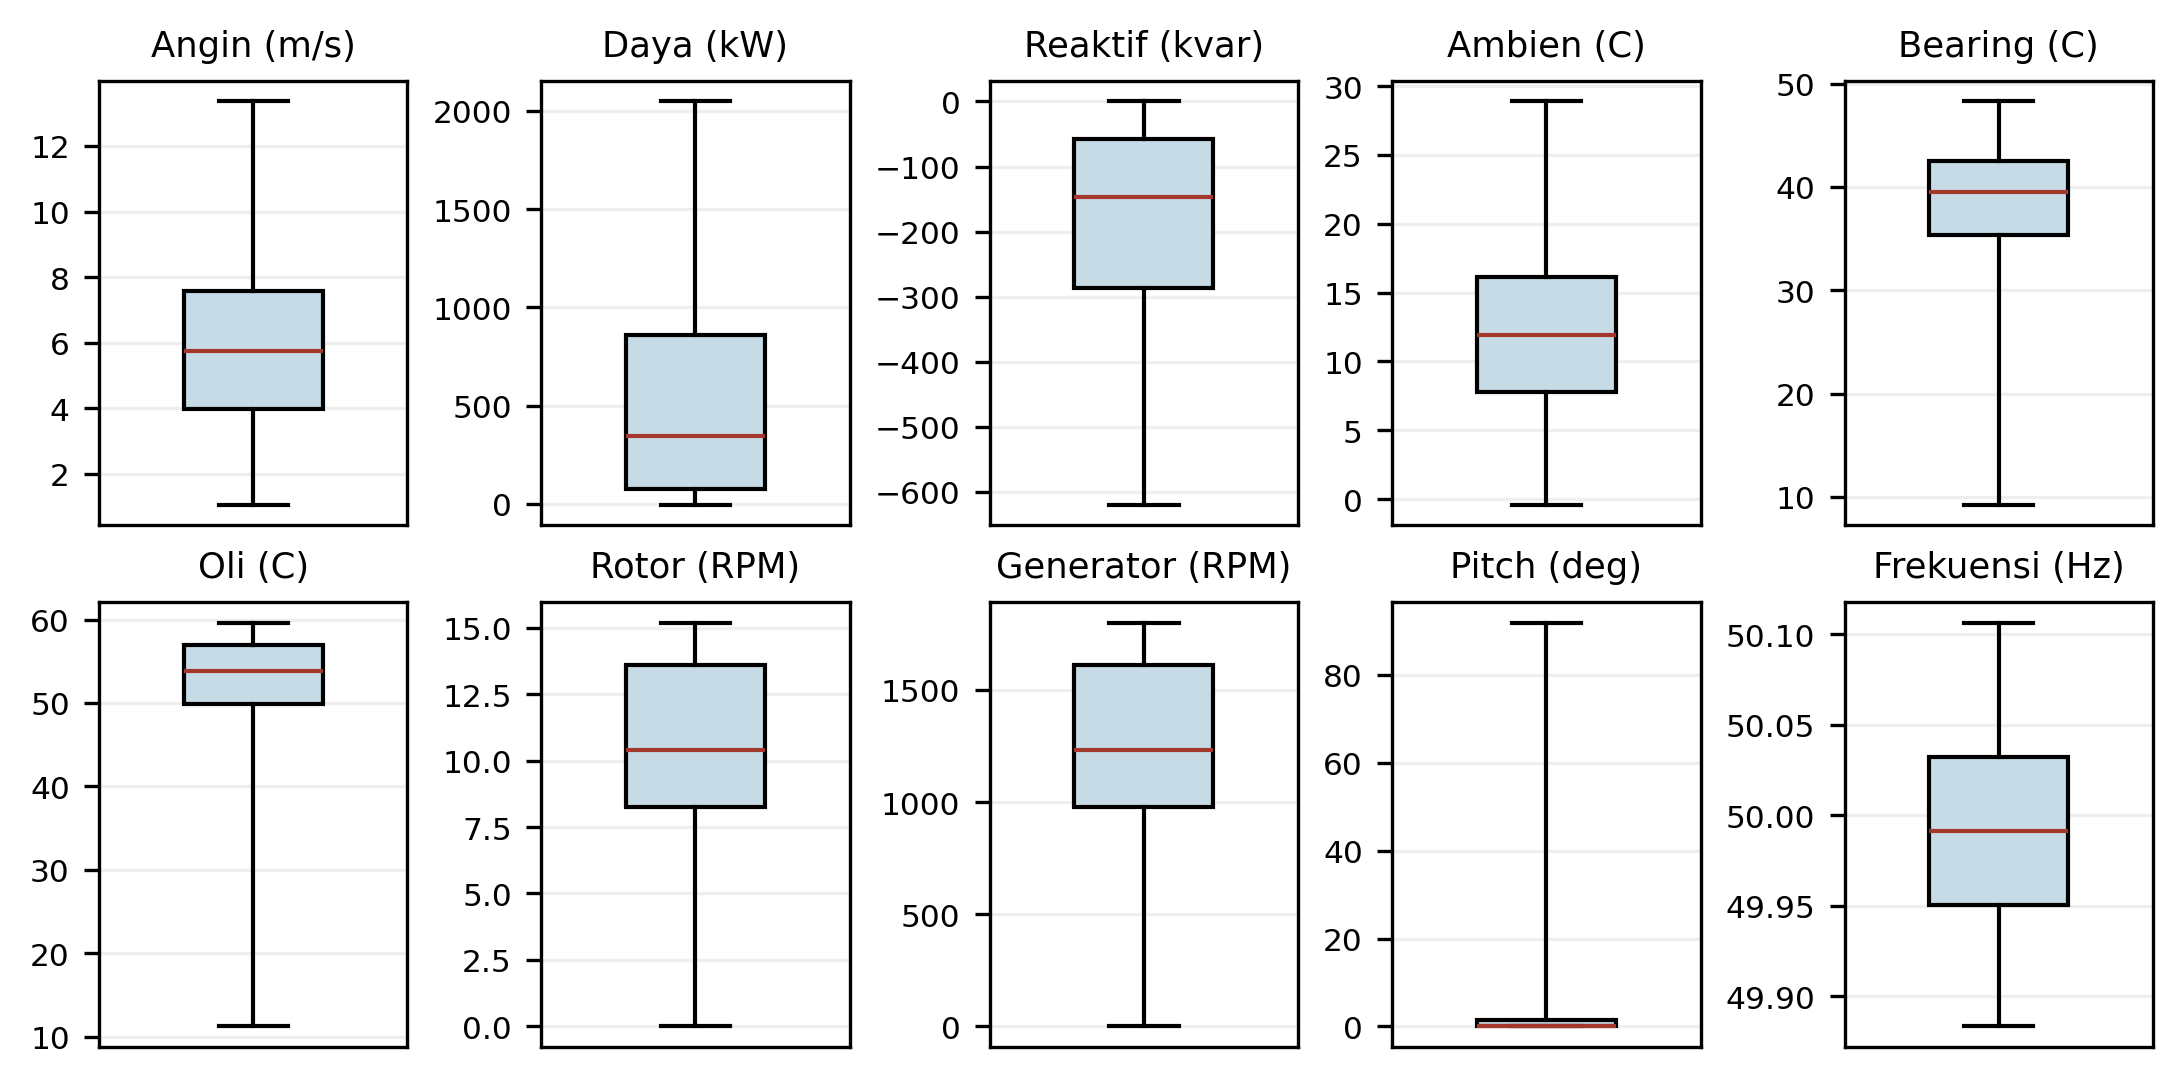
\includegraphics[width=0.68\columnwidth]{sensor_quantiles.png}
\caption{Sebaran kuantil sinyal terpilih (P1/P99 sebagai whisker, bukan pagar Tukey).}
\label{fig:quantiles}
\end{figure}

Ketergantungan temporal diringkas pada Tabel~\ref{tab:autocorr} untuk satu turbin (KWF1). Autokorelasi, yaitu korelasi sinyal dengan dirinya pada lag tertentu, tetap tinggi pada lag 10 menit (angin 0,966; daya 0,966; ambien 0,999), dan ambien masih 0,901 pada 24 jam karena siklus harian. Observasi berurutan karenanya tidak independen, sehingga representasi window dan pembagian waktu kronologis diperlukan \cite{martipuig2024,draayer2026,lang2026,bette2023}.

\begin{table}[!t]
\centering
\caption{Autokorelasi KWF1 pada lag 10 menit, 1 jam, dan 24 jam.}
\label{tab:autocorr}
\footnotesize
\setlength{\tabcolsep}{4pt}
\begin{tabular}{lrrr}
\toprule
Sinyal & 10 menit & 1 jam & 24 jam \\
\midrule
Angin & 0,966 & 0,894 & 0,412 \\
Daya & 0,966 & 0,885 & 0,420 \\
Ambien & 0,999 & 0,991 & 0,901 \\
Bearing & 0,980 & 0,812 & 0,455 \\
\bottomrule
\end{tabular}
\end{table}

\subsection{Skala, korelasi, dan keputusan preprocessing}
Gambar~\ref{fig:geom_a} merangkum ketimpangan skala pada audit sebelum clustering. Simpangan baku generator 538,15 RPM berbeda secara numerik sekitar 1.478 kali dari frekuensi 0,36409 Hz; daya aktif mencapai 593,34 kW. Satuan yang berbeda menjelaskan dominasi jarak mentah, bukan perbandingan energi antarbesaran. Median daya 347,36 kW lebih kecil dari mean 559,55 kW; pitch memiliki Q1 nol, median 0,10, Q3 1,49, tetapi persentil 99 sebesar 91,94 derajat. IQR pitch yang kecil di pusat sebaran dapat memperbesar bobot ekornya pada RobustScaler.

\begin{figure}[H]
\centering
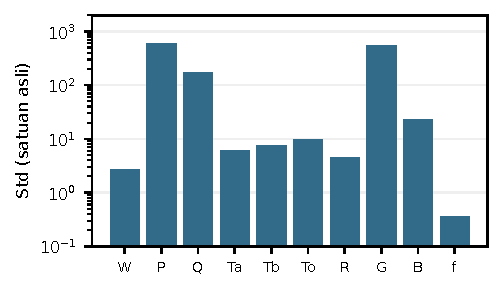
\includegraphics[width=0.48\columnwidth]{geom_a.pdf}
\caption{Simpangan baku sinyal terpilih pada satuan asli (sumbu log). W/P/Q: angin/daya aktif/reaktif; Ta/Tb/To: ambien/bearing/oli; R/G: rotor/generator; B: pitch; f: frekuensi.}
\label{fig:geom_a}
\end{figure}

Pearson rotor--generator 0,99998, angin--daya 0,88293, dan reaktif--aktif $-0,88362$ menunjukkan bobot informasi berulang (Gambar~\ref{fig:geom_b}), sejalan dengan perlunya audit korelasi SCADA \cite{bette2023}. Standardisasi tidak menghilangkan redundansi. Pemeriksaan 60 fitur window menemukan 38 pasangan dengan $|r|\ge0,95$, terutama antarstatistik sinyal yang sama; pembuangan fitur redundan diuji pada Subbagian kontrol. Sinyal tetap dipertahankan agar seluruh kandidat menerima fitur yang sama; sensitivitas bobot diperiksa terpisah.

\begin{figure}[H]
\centering
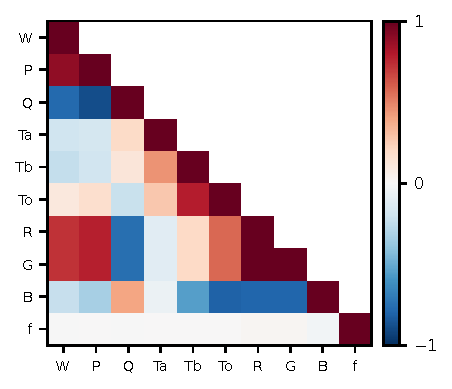
\includegraphics[width=0.48\columnwidth]{geom_b.pdf}
\caption{Korelasi Pearson sensor skalar yang tersimpan.}
\label{fig:geom_b}
\end{figure}

Kontribusi maksimum jarak (Gambar~\ref{fig:geom_c}) berubah dari 48,90\% tanpa scaling menjadi 44,87\% Standard, 22,65\% Min--Max, dan 61,72\% Robust (pitch); dominasi Robust berkaitan dengan ekor dan IQR sempit. Stress-test satu ekstrem sintetis menyisakan 28,06\% jarak pada Standard, 0,62\% Min--Max, dan hampir 100\% Robust. Standard adalah kompromi, tetap sensitif terhadap ekstrem dan tidak terbukti lebih baik untuk skor clustering.

\begin{figure}[H]
\centering
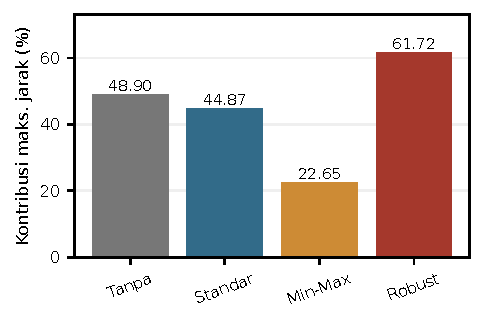
\includegraphics[width=0.48\columnwidth]{geom_c.pdf}
\caption{Kontribusi maksimum sensor pada jarak kuadrat tiap scaler.}
\label{fig:geom_c}
\end{figure}

Gambar~\ref{fig:qual_a} dan Gambar~\ref{fig:qual_b} membedakan kehilangan slot dari missingness sensor. Cakupan total 99,57\% menyembunyikan slot tidak tersedia 1,054\% pada KWF1 versus 0,137\% pada KWF2; celah terpanjang mencapai 48,83 jam. Missingness ambien/pitch/setpoint pada baris tersedia sekitar 0,082\%. Mengisi 19 sel ambien tidak memulihkan gap panjang. IQR trimming pada benchmark akan menghapus 22,56\% slot seleksi dan seluruh subset low-power/high-wind yang didefinisikan untuk screening; subset tersebut bukan label kondisi tervalidasi. Flag-only mempertahankan nilai dan menghindari kesimpulan otomatis bahwa ekor adalah error.

\begin{figure}[H]
\centering
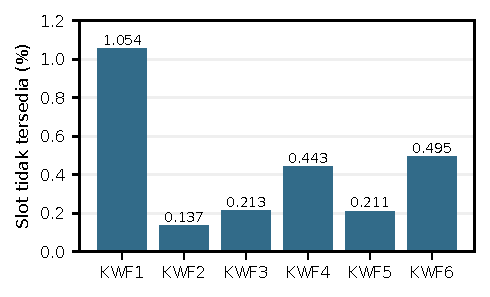
\includegraphics[width=0.48\columnwidth]{qual_a.pdf}
\caption{Fraksi slot tanpa availability=1 per turbin.}
\label{fig:qual_a}
\end{figure}

\begin{figure}[H]
\centering
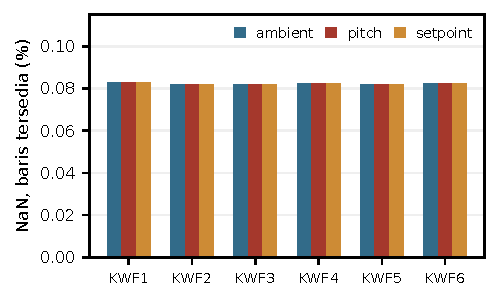
\includegraphics[width=0.48\columnwidth]{qual_b.pdf}
\caption{Missingness sensor pada baris tersedia (setpoint hanya konteks).}
\label{fig:qual_b}
\end{figure}

Pada kelengkapan 100\%, retensi window seleksi adalah 99,49\% (1 jam), 98,96\% (6 jam), dan 97,37\% (24 jam) (Gambar~\ref{fig:qual_c}). Satu slot hilang dari enam memberi kelengkapan 83,33\%, sehingga threshold 90/95/100\% menghasilkan window satu jam yang sama. Durasi terpendek memenuhi aturan retensi, tetapi grafik bukan perbandingan kualitas clustering. Hasilnya 25.881 training dan 26.360 seleksi (52.241 window, 60 fitur finite, keys unik). PFA 32 fitur mempertahankan korelasi jarak 0,99415; input utama tetap 60 fitur bernama tanpa reduksi.

\begin{figure}[H]
\centering
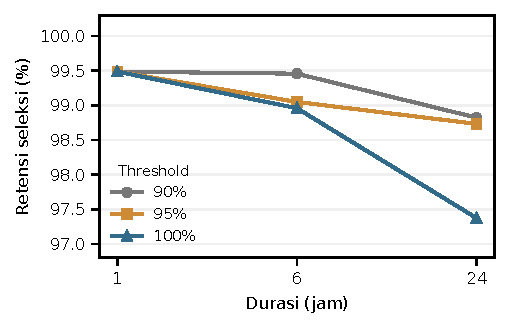
\includegraphics[width=0.48\columnwidth]{qual_c.pdf}
\caption{Retensi window Juli--Desember pada threshold 90/95/100\%.}
\label{fig:qual_c}
\end{figure}

\subsection{K-Means++ dan ringkasan dengan cakupan penuh}
\begin{table}[!t]
\centering
\caption{K-Means++ pada 26.360 window seleksi; Silhouette pada sampel 3.000 yang sama.}
\label{tab:kmeans}
\footnotesize
\setlength{\tabcolsep}{3pt}
\begin{tabular}{rrrrr}
\toprule
$k$ & Silhouette & DBI & CHI & Minimum ($n$) \\
\midrule
2 & 0,32954 & 1,856 & 4071,3 & 5396 \\
3 & 0,15964 & 1,753 & 3303,3 & 2727 \\
4 & 0,17732 & 1,782 & 3049,0 & 1323 \\
5 & 0,18086 & 1,484 & 3635,9 & 4 \\
6 & 0,12510 & 1,754 & 3193,3 & 4 \\
7 & 0,13537 & 1,768 & 2909,6 & 4 \\
8 & 0,10354 & 1,908 & 2661,3 & 4 \\
9 & 0,11437 & 1,847 & 2529,2 & 4 \\
10 & 0,11848 & 1,813 & 2356,5 & 4 \\
\bottomrule
\end{tabular}
\end{table}

Tabel~\ref{tab:kmeans} dan Gambar~\ref{fig:sil} menunjukkan penurunan separasi dari $k=2$ ke $k=3$, bukan peningkatan otomatis saat granularitas bertambah. $k=2$ memberi Silhouette/CHI tertinggi, kelompok terkecil 20,47\%, ARI seed 1,00, dan persistence seleksi 0,93353. DBI terbaik justru $k=5$ (1,48402), tetapi kelompok terkecil hanya empat window (0,01517\%). Kelompok langka tetap dicatat, tanpa disebut fault. Perbedaan arah indeks mengharuskan pemeriksaan ukuran/profil; $k=2$ dipilih untuk ringkasan stabil dengan cakupan seluruh window, bukan jumlah kondisi sejati atau pemenang universal. Inertia, yaitu jumlah kuadrat jarak ke centroid, menurun dari $1,258\times10^6$ ($k=2$) ke $6,99\times10^5$ ($k=10$) tanpa siku tajam; pemilihan $k$ karena itu bertumpu pada indeks validitas, bukan Elbow semata.

\begin{figure}[H]
\centering
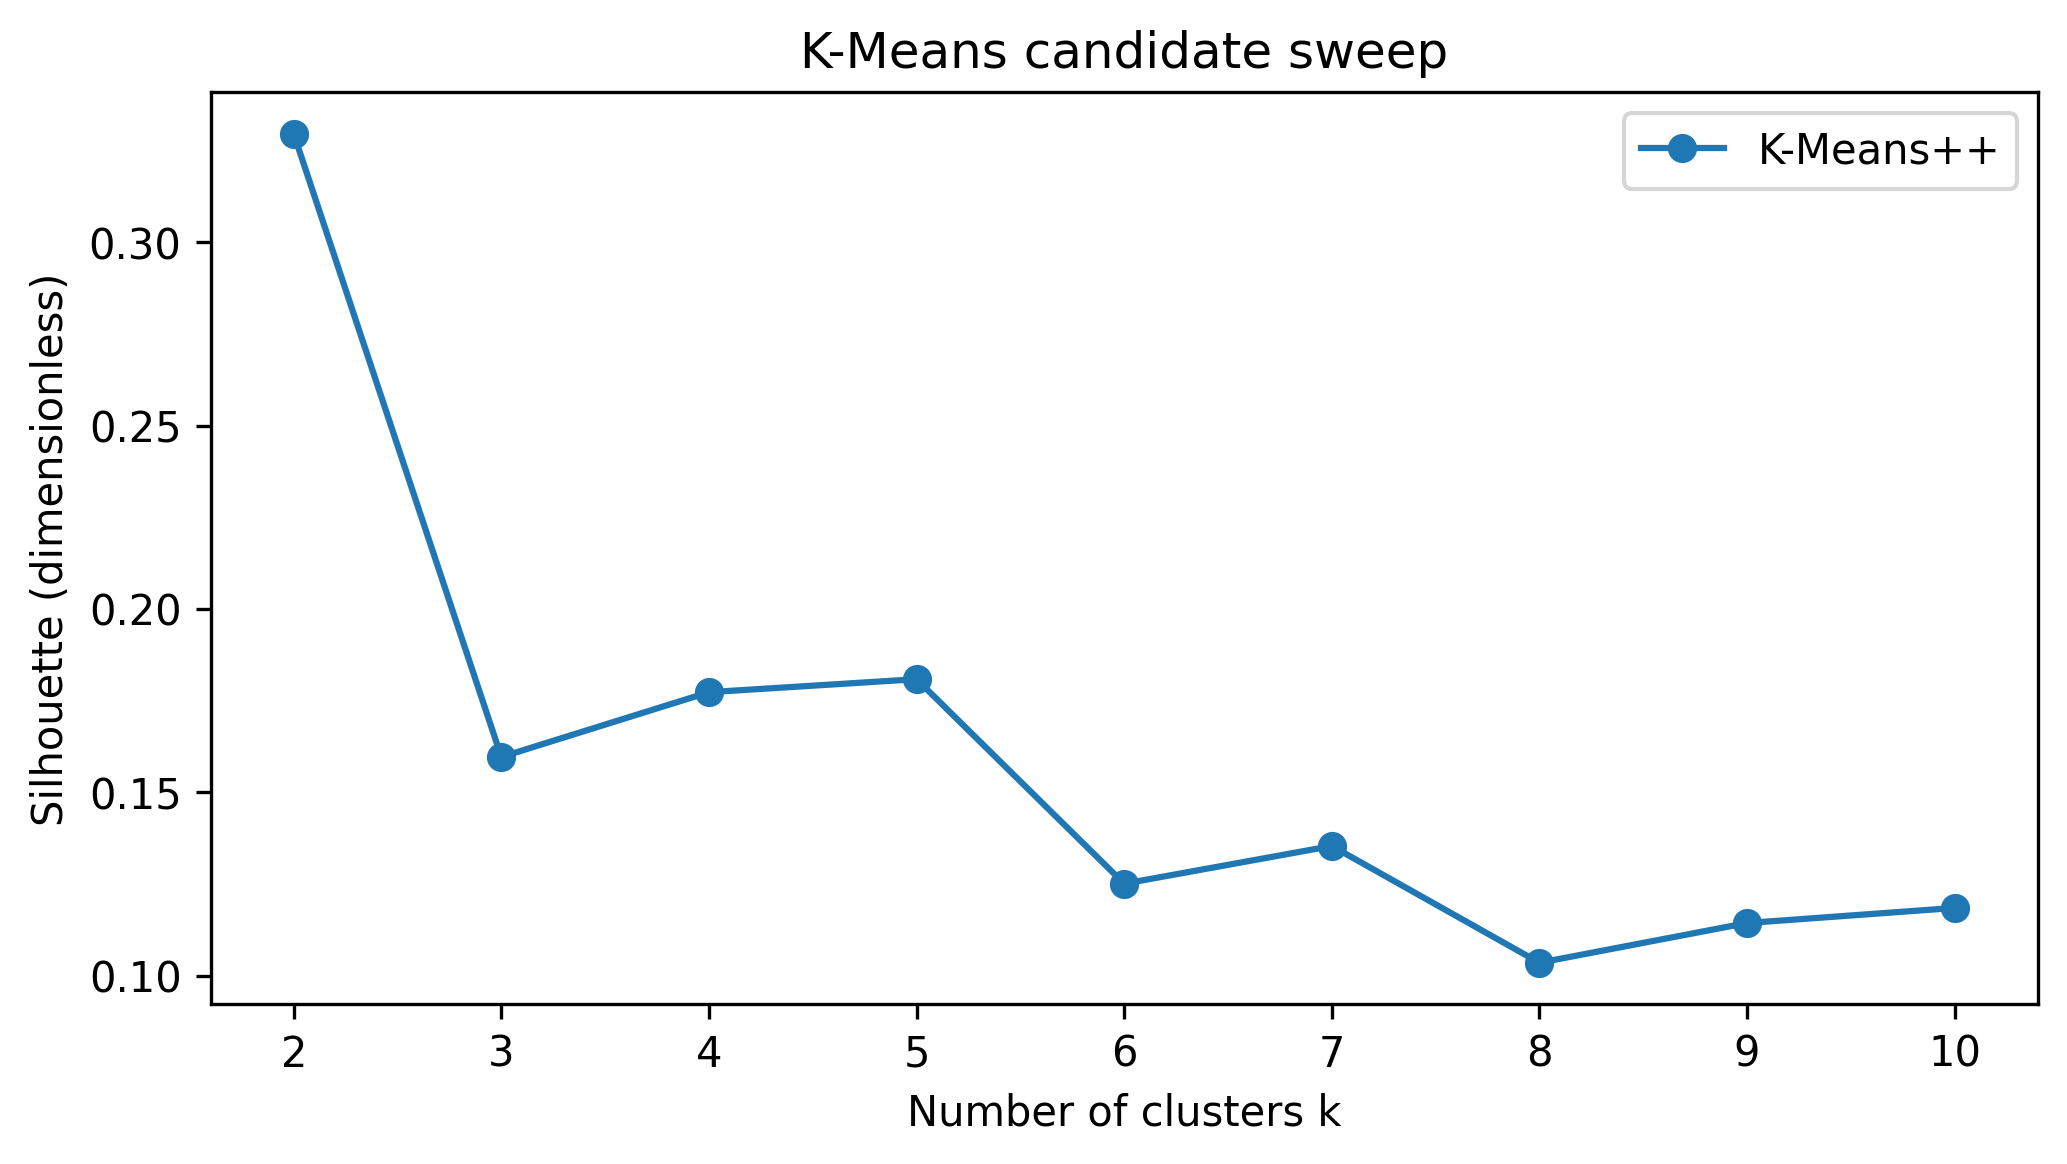
\includegraphics[width=0.72\columnwidth]{k_silhouette.png}
\caption{Sweep Silhouette pada sampel seleksi yang sama.}
\label{fig:sil}
\end{figure}

\subsection{FCM, HDBSCAN, dan sensitivitas Ward}
FCM standar $m=2$ pada $k=2$--10 mengalami pusat hampir berimpit, FPC mendekati $1/k$, entropi ternormalisasi mendekati 1, dan keanggotaan maksimum di bawah 0,60; hard assignment mengisi hanya dua label pada $k>2$. Tiga dari 45 inisialisasi (seed 2026, $k=4,5,6$) mencapai batas 500 iterasi, tetapi tiap $k$ tetap punya inisialisasi konvergen. ARI seed tinggi tidak memperbaiki keanggotaan seragam, dan label argmax dapat mencerminkan selisih numerik kecil. Penyebab kausal collapse belum diuji; hasil tidak membatalkan semua keluarga fuzzy \cite{cai2025}.

\begin{table}[H]
\centering
\caption{Metrik kandidat pada populasi evaluasinya; $N$ objek, Silhouette dari subset tetap (penuh 3.000; non-noise 1.969).}
\label{tab:compare}
\footnotesize
\setlength{\tabcolsep}{4pt}
\begin{tabularx}{\columnwidth}{@{}P{.42\columnwidth}rrrr@{}}
\toprule
\textbf{Metode (populasi)} & $N$ & Sil. & DBI & CHI \\
\midrule
K-Means $k{=}2$ (seleksi penuh) & 26360 & 0,3295 & 1,856 & 4071 \\
FCM $k{=}2$ (argmax) & 26360 & 0,1203 & 2,135 & 3122 \\
HDBSCAN c800/s10 (non-noise) & 17847 & 0,4382 & 1,076 & 3496 \\
K-Means $k{=}2$ (non-noise sama) & 17847 & 0,4059 & 1,298 & 3281 \\
Ward $k{=}2$ (sampel training) & 4000 & 0,3644 & 1,303 & 892 \\
K-Means $k{=}2$ (sampel sama) & 4000 & 0,3238 & 1,680 & 1007 \\
\bottomrule
\end{tabularx}
\end{table}

Enam konfigurasi HDBSCAN membentuk 2--3 kelompok dengan cakupan 64,95--67,70\% dan noise 32,30--35,05\%. Tabel~\ref{tab:compare} menunjukkan tiga indeks conditional lebih baik daripada K-Means ketika 17.847 objek dan 1.969 sampel Silhouette disamakan; ARI partisi 0,87643. Keuntungan itu tidak menghilangkan 8.513 window yang ditolak c800/s10. c300/s30 dan c800/s30 memberi Silhouette lebih tinggi (0,45891), tetapi cakupan lebih kecil (65,19\%); anggotanya berubah. ARI common-assigned minimum 0,99478 menunjukkan inti konsisten antarkonfigurasi, bukan validitas noise.

Noise c800/s10 mempunyai median daya 92,86 kW dan rotor 8,09 RPM; inti memisahkan daya 428,10/$-1,65$ kW dan rotor 11,01/0,03 RPM. Noise bukan satu state fisik. Persistence assigned-only 0,99718 mengecualikan 43,51\% pasangan yang menyentuh noise, sehingga tidak disetarakan dengan persistence K-Means penuh. HDBSCAN tetap dipertahankan sebagai pembanding struktur inti, tanpa klaim cakupan penuh.

Ward $k=2$ pada Tabel~\ref{tab:compare} mempunyai Silhouette/DBI lebih baik daripada K-Means pada sampel training yang sama, tetapi CHI lebih rendah dan ARI antarmetode hanya 0,56701. Profil median daya Ward 505,85/$-1,25$ kW, rotor 11,44/0,03 RPM, serta pitch 0,14/89,99 derajat mendukung pemisahan besar dengan batas berbeda. Sweep Ward $k=2$--10 tetap merupakan sensitivity check; tidak ada evaluasi prediksi seleksi Ward.

\subsection{Profil refit dan batas interpretasi}
Setelah kandidat dan profil diperiksa, K-Means++ $k=2$ telah di-fit ulang pada seluruh tahun dengan scaler tetap. Ukuran akhir 10.405 (19,92\%) dan 41.836 (80,08\%); ARI terhadap assignment kandidat pada window sama 0,98129. Karena model berubah, skor seleksi tidak dinyatakan sebagai skor refit.

\begin{table}[H]
\centering
\caption{Median mean per window, model refit seluruh tahun.}
\label{tab:profiles}
\footnotesize
\setlength{\tabcolsep}{3pt}
\begin{tabular}{lrr}
\toprule
Sensor (satuan) & Klaster 0 & Klaster 1 \\
\midrule
Angin (m/s) & 2,746 & 6,262 \\
Daya aktif (kW) & $-0,840$ & 515,589 \\
Reaktif (kvar) & $-0,027$ & $-192,641$ \\
Rotor (RPM) & 1,359 & 11,562 \\
Generator (RPM) & 162,300 & 1371,292 \\
Pitch (derajat) & 41,728 & 0,056 \\
Ambien ($^\circ$C) & 13,397 & 11,599 \\
Bearing ($^\circ$C) & 38,207 & 39,967 \\
Oli ($^\circ$C) & 43,233 & 55,047 \\
Frekuensi (Hz) & 49,993 & 49,991 \\
\bottomrule
\end{tabular}
\end{table}

Tabel~\ref{tab:profiles} menunjukkan kelompok 0 dengan daya/putaran rendah dan pitch lebih besar; kelompok 1 dengan produksi/putaran lebih tinggi. Perbedaan oli memberi deskripsi tambahan, tetapi tidak menetapkan sebab termal. Gambar~\ref{fig:wp} memperlihatkan tumpang tindih pada proyeksi angin--daya karena label dibentuk dari 60 koordinat; batas bukan threshold dua sensor saja. Kelompok bukan label normal, shutdown, curtailment, atau fault tanpa ground truth.

\begin{figure}[H]
\centering
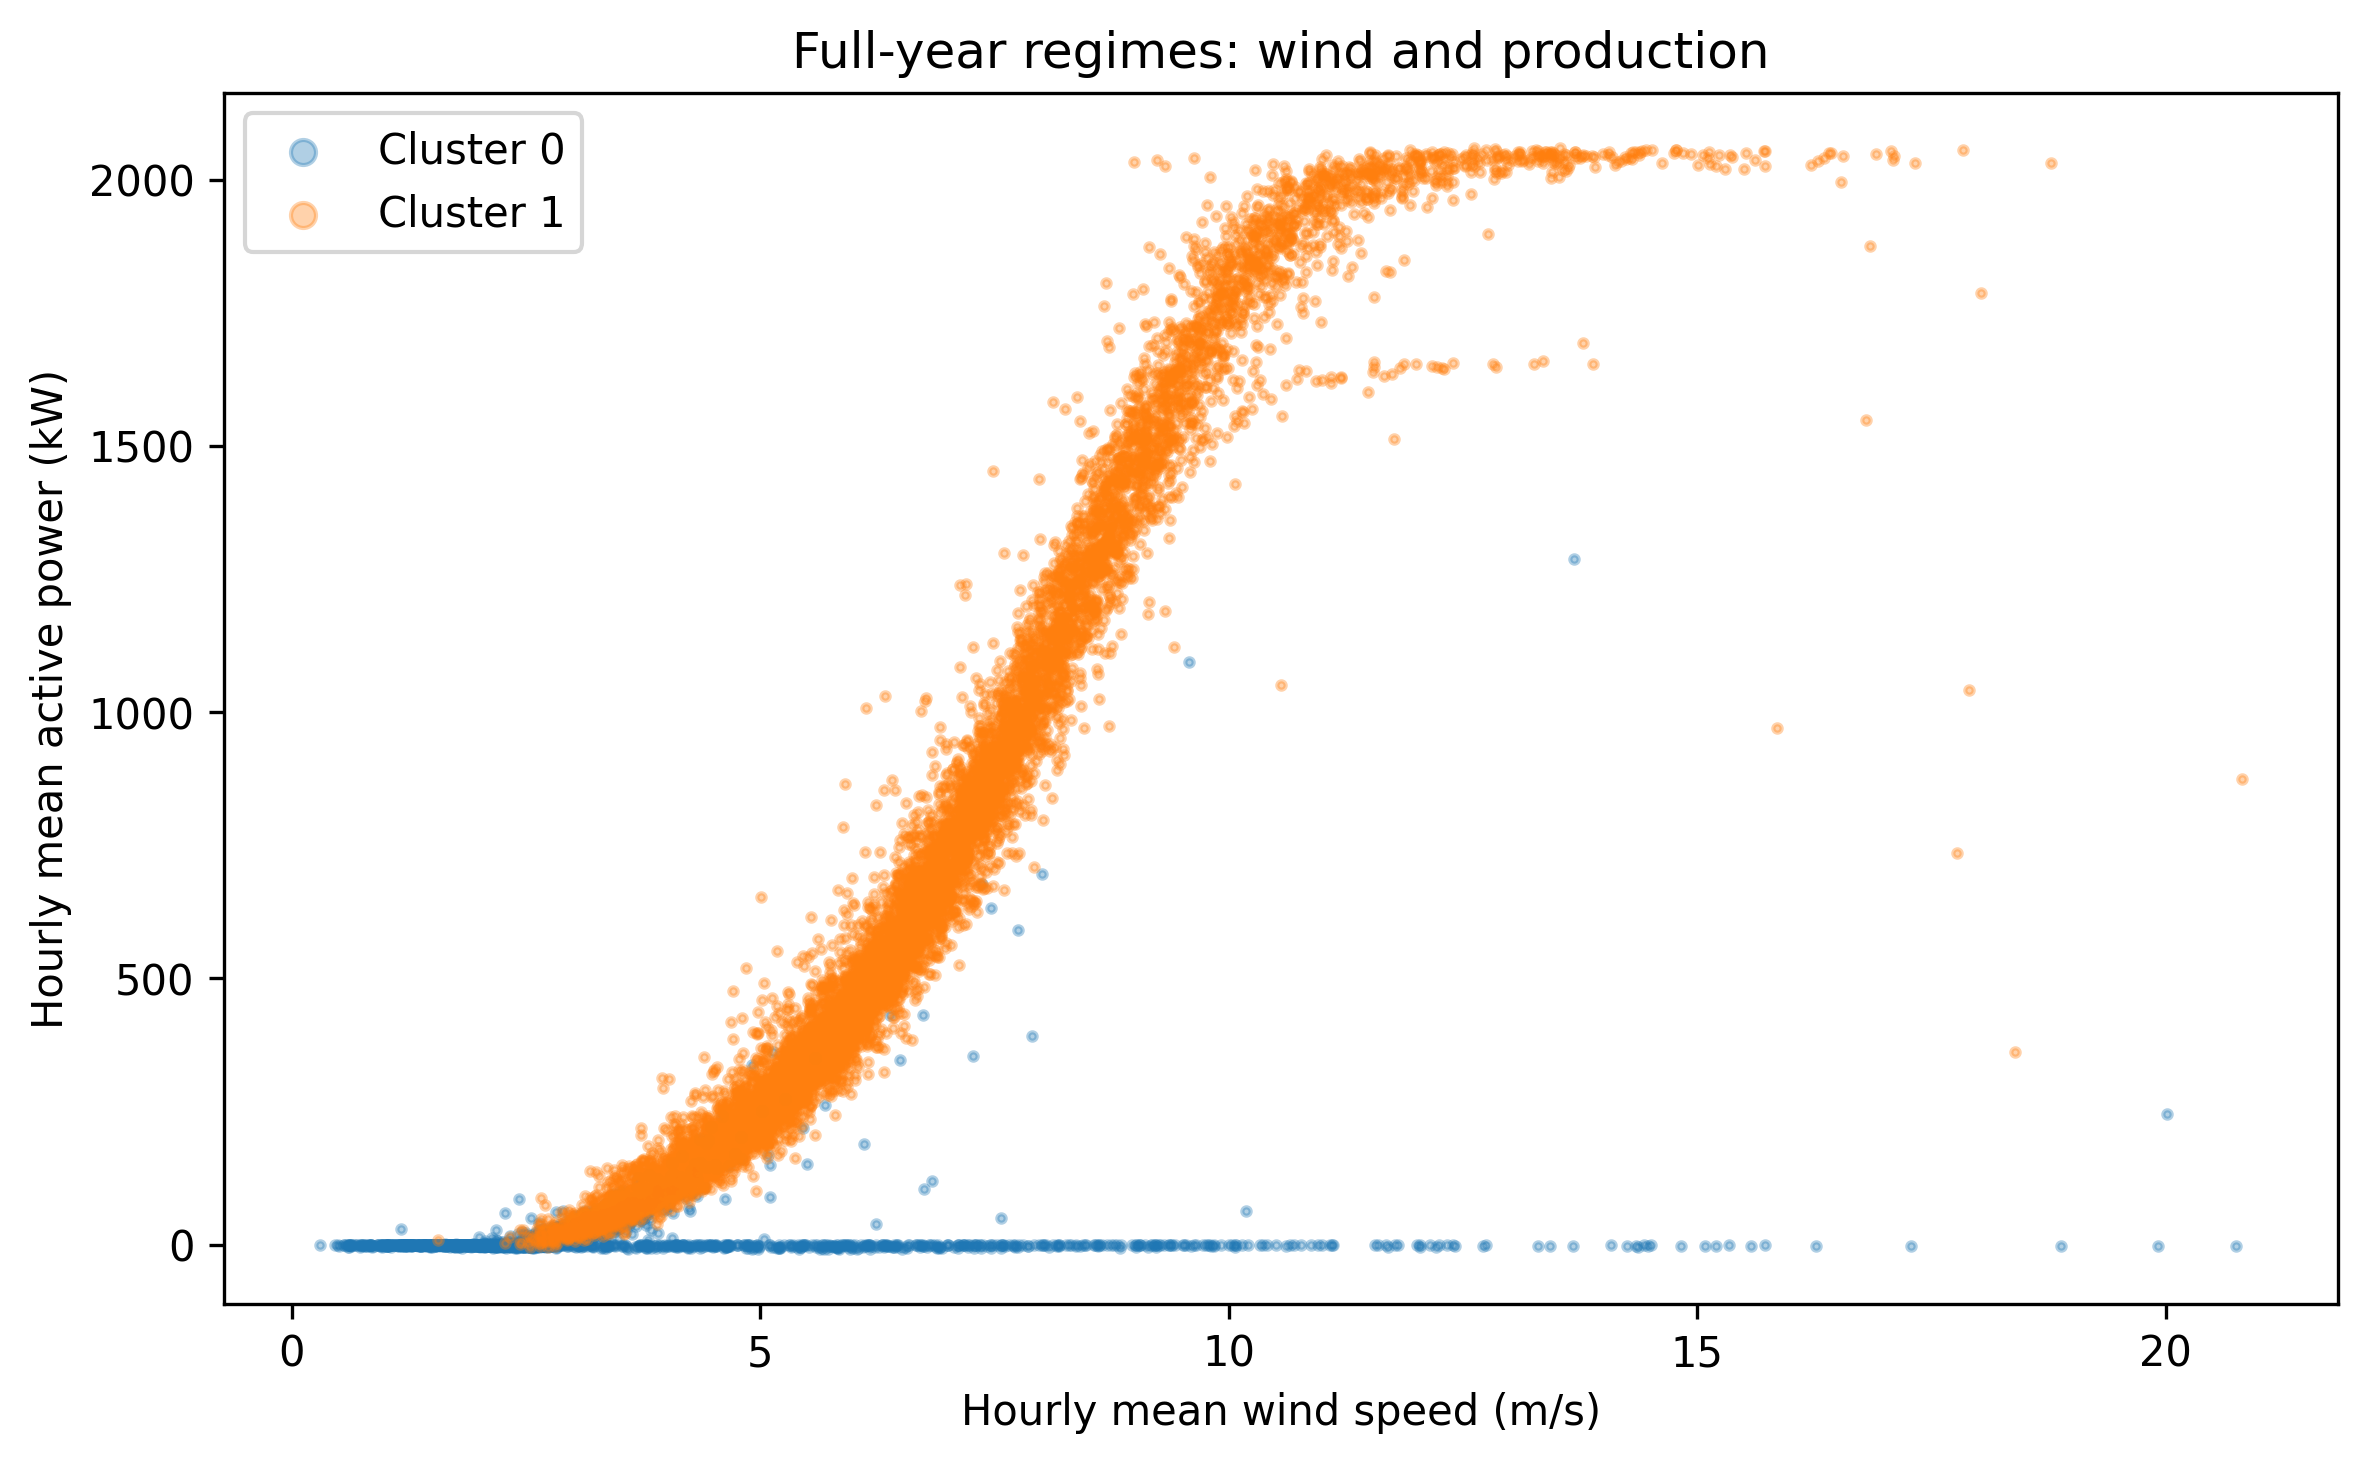
\includegraphics[width=0.72\columnwidth]{wind_power.png}
\caption{Sampel deterministik 12.000 window (seed 2022) dari assignment refit seluruh tahun pada mean fisik angin--daya.}
\label{fig:wp}
\end{figure}

Persistence refit 0,93400 pada 52.170 pasangan satu jam tetap memutus batas turbin, split, dan gap. NMI terhadap identitas turbin 0,00231 rendah, bukan bukti kebenaran operasi. Mean rotor--generator pada training berkorelasi 0,999992; sensitivitas bobot keluarga rotor/generator $1/\sqrt2$ memberi ARI 0,98188 ($k=2$). Sebanyak 1\% norma terbesar menyumbang 11,79\% jumlah kuadrat norma training. Kedua diagnostik memberi konteks geometri tanpa mengganti input utama atau membuktikan sebab kegagalan FCM.

\subsection{Kontrol preprocessing dan representasi temporal}
Tabel~\ref{tab:rq1} merangkum kontrol satu faktor pada populasi seleksi; referensi StandardScaler dengan 60 fitur memberi Silhouette 0,3293 dan DBI 1,8568. Faktor skala paling menggeser struktur: tanpa scaling partisi berubah hampir total (ARI $-0,054$) dan terpisah menurut besaran sensor berskala besar, bukan rezim operasi; RobustScaler memberi Silhouette 0,838 tetapi hanya mengisolasi kelompok $3,5\%$ (ARI 0,172), sedangkan standardisasi per-turbin hampir tidak mengubah partisi (ARI 0,931). Pada faktor redundansi, pembuangan keluarga generator (ARI 0,982) dan frekuensi (ARI 0,9997) nyaris tidak mengubah struktur, sedangkan representasi 12 mean mempertegas geometri (Silhouette 0,414, DBI 1,291) dengan interpretasi idle--produksi yang sama. Faktor ekstrem (winsor) dan kebijakan missing hanya menggeser struktur sedikit (ARI $\geq0,977$).

\begin{table}[H]
\centering
\caption{Kontrol satu faktor preprocessing; ARI terhadap referensi.}
\label{tab:rq1}
\footnotesize
\setlength{\tabcolsep}{4pt}
\begin{tabular}{llrrr}
\toprule
Faktor & Varian & Sil. & DBI & ARI \\
\midrule
Skala & tanpa scaling & 0,468 & 0,807 & $-0,054$ \\
Skala & RobustScaler & 0,838 & 0,385 & 0,172 \\
Skala & Min--Max & 0,221 & 1,563 & 0,111 \\
Skala & per-turbin & 0,369 & 1,895 & 0,931 \\
Redundansi & 12 mean & 0,414 & 1,291 & 0,823 \\
Redundansi & buang generator & 0,308 & 1,983 & 0,982 \\
Redundansi & level $+$ dinamika & 0,336 & 1,896 & 0,769 \\
Redundansi & buang frekuensi & 0,317 & 1,784 & 1,000 \\
Ekstrem & winsor 1--99 & 0,282 & 1,863 & 0,992 \\
Ekstrem & winsor 5--95 & 0,259 & 1,812 & 0,977 \\
\bottomrule
\end{tabular}
\end{table}

Kontrol representasi temporal (Tabel~\ref{tab:rq2}) menunjukkan kedua representasi menemukan rezim yang sama (idle sekitar $16\%$ versus produksi), dengan ARI antara label window dan pointwise 0,850 dan kecocokan mentah 96,9\%. Perbedaan utamanya koherensi: pointwise berganti label $1,16$ kali per jam dengan median run $0,5$ jam, sedangkan window satu jam berganti $0,31$ kali per jam dengan median run $4$ jam. Agregasi temporal karena itu tidak mengubah identitas rezim kasar, tetapi menstabilkan label; Silhouette pointwise yang sedikit lebih tinggi (0,430) tidak diartikan lebih bermakna karena objek dan granularitasnya berbeda.

\begin{table}[H]
\centering
\caption{Pointwise 10 menit versus window 1 jam pada 12 sinyal.}
\label{tab:rq2}
\footnotesize
\setlength{\tabcolsep}{4pt}
\begin{tabular}{lrr}
\toprule
 & Pointwise & Window \\
\midrule
Objek & 314.018 & 52.241 \\
Silhouette & 0,430 & 0,414 \\
DBI & 1,226 & 1,291 \\
Idle (\%) & 15,5 & 16,6 \\
Run rata-rata (jam) & 5,13 & 18,96 \\
Run median (jam) & 0,50 & 4,00 \\
Ganti label per jam & 1,159 & 0,308 \\
\bottomrule
\end{tabular}
\end{table}

\subsection{Keterbatasan}
NMI kandidat dengan any IQR flag 0,57997 dan physical flag 0,10440 perlu dibaca hati-hati: flag dibentuk dari sensor yang juga menentukan klaster, sehingga asosiasi dapat bersifat sirkular. Label independen tidak tersedia; event 69.850 baris hanya konteks yang belum menjadi validasi state. Ketergantungan waktu, satu lokasi/tahun, penggunaan ulang periode seleksi, redundansi statistik, dan hilangnya transien pada agregasi 10 menit membatasi generalisasi. Kontrol scaler, redundansi, ekstrem, dan kebijakan missing serta representasi pointwise-versus-window telah dilaporkan pada Subbagian sebelumnya; validasi konteks status dan durasi window lain di luar cakupan.

\section{Kesimpulan dan saran}
Input beku 52.241 window dan 60 fitur mendukung K-Means++ $k=2$ sebagai ringkasan deskriptif cakupan penuh (Silhouette 0,32954, DBI 1,85605, CHI 4071,28, ARI seed 1,00); profil refit dibedakan oleh daya, putaran, dan pitch. FCM standar degeneratif pada pengaturan yang diuji; HDBSCAN informatif untuk inti padat dengan cakupan parsial; Ward menunjukkan sensitivitas batas kelompok, dan metrik dari populasi berbeda tidak diranking bersama. Kontrol satu faktor menunjukkan pilihan skala paling menentukan struktur (tanpa scaling ARI $-0,054$; standardisasi per-turbin 0,931), sedangkan pembuangan fitur redundan, winsorization, dan kebijakan missing hanya menggeser sedikit; representasi 12 mean mempertegas geometri (Silhouette 0,414) dengan rezim yang sama. Representasi temporal tidak mengubah identitas rezim (ARI 0,85) tetapi menstabilkan label (median run 0,5 menjadi 4 jam). Pengujian tahun/lokasi lain serta validasi konteks status tetap diperlukan; penelitian ini tidak mengklaim label kondisi terverifikasi.

\begin{thebibliography}{21}

\bibitem{kelmarsh2025}
C. Plumley and R. Takeuchi, ``Kelmarsh wind farm data,'' Zenodo, ver. 4, Aug. 12, 2025, doi: 10.5281/zenodo.16807551.

\bibitem{martipuig2024}
P. Marti-Puig and C. N{\'u}{\~n}ez-Vilaplana, ``Dynamic Clustering of Wind Turbines Using SCADA Signal Analysis,'' \textit{Energies}, vol. 17, no. 11, Art. no. 2514, 2024, doi: 10.3390/en17112514.

\bibitem{bonifati2022}
A. Bonifati, F. Del Buono, F. Guerra, and D. Tiano, ``Time2Feat: Learning Interpretable Representations for Multivariate Time Series Clustering,'' \textit{Proc. VLDB Endow.}, vol. 16, no. 2, pp. 193--201, 2022, doi: 10.14778/3565816.3565822.

\bibitem{ngophan2025}
Q.-D. Ngo and L.-H. Phan, ``Analysis of Multivariate Indoor Building Data: A Comparative Study of Time-Series Clustering Methods,'' \textit{IEEE Access}, vol. 13, pp. 139018--139032, 2025, doi: 10.1109/ACCESS.2025.3596297.

\bibitem{mazgula2024}
J. Mazgu{\l}a, D. Kr{\'o}l, and I. Jab{\l}o{\'n}ski, ``Temporal and Multivariate Similarity Clustering of 5G Performance Data,'' \textit{IEEE Access}, vol. 12, pp. 114137--114145, 2024, doi: 10.1109/ACCESS.2024.3444704.

\bibitem{cai2025}
C. Cai, Q. Shi, X. Cheng, Y. Tao, and S. Hou, ``Short-Term Offshore Wind Power Forecasting Based on Dynamic Trend Clustering of Meteorological Factors,'' \textit{IEEE Trans. Instrum. Meas.}, vol. 74, pp. 1--16, 2025, doi: 10.1109/TIM.2025.3613908.

\bibitem{ghaderi2023}
H. Ghaderi, B. Foreman, A. Nayebi, S. Tipirneni, C. K. Reddy, and V. Subbian, ``A self-supervised learning-based approach to clustering multivariate time-series data with missing values (SLAC-Time): An application to TBI phenotyping,'' \textit{J. Biomed. Inform.}, vol. 143, Art. no. 104401, 2023, doi: 10.1016/j.jbi.2023.104401.

\bibitem{draayer2026}
E. Draayer, H. Cao, and Q. Gong, ``Deep clustering for large-scale interpretable time series segmentation,'' \textit{Data Min. Knowl. Discov.}, vol. 40, Art. no. 2, 2026, doi: 10.1007/s10618-025-01170-y.

\bibitem{belhadj2026}
Y. Bel-Hadj, F. de Nolasco Santos, W. Weijtjens, and C. Devriendt, ``Inferring wind turbine operational state and fatigue from high-frequency acceleration using self-supervised learning for SCADA (supervisory control and data acquisition)-free monitoring,'' \textit{Wind Energ. Sci.}, vol. 11, pp. 1363--1382, 2026, doi: 10.5194/wes-11-1363-2026.

\bibitem{lang2026}
X. Lang, M. Zhang, and W. Mao, ``Data-driven segmentation of ship operational conditions using multivariate time-series clustering,'' \textit{Ships Offshore Struct.}, published online Jul. 6, 2026, doi: 10.1080/17445302.2026.2699360.

\bibitem{bette2023}
H. M. Bette, E. Jungblut, and T. Guhr, ``Nonstationarity in correlation matrices for wind turbine SCADA-data,'' \textit{Wind Energy}, vol. 26, no. 8, pp. 826--849, 2023, doi: 10.1002/we.2843.

\bibitem{li2026}
H. Li and J. Li, ``Research on SCADA Data Preprocessing Method for Wind Turbines Based on Variable Grid Optimization (VGO-K-Means),'' \textit{Electronics}, vol. 15, no. 14, Art. no. 3078, 2026, doi: 10.3390/electronics15143078.

\end{thebibliography}

\end{document}
